\subsection{Results of our Corner-based Point Matching}
% Image 1
\begin{figure}[H]\centering
	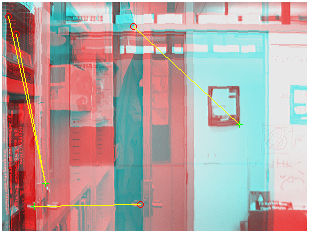
\includegraphics[width=0.8\linewidth]{Images/01_matlab_match.png}
	\caption{Interesting points and matches found using MATLAB's implementation on Image 1.}
	\label{fig:jp-ofc-matlab-match}
\end{figure}

\begin{figure}[H]\centering
	
\includegraphics[width=0.8\linewidth]{Images/01_matlab_depth.png}
	\caption{Depth map using the interesting points and matches using MATLAB's implementation on Image 1.}
	\label{fig:jp-ofc-matlab-depth}
\end{figure}

\begin{figure}[H]\centering
	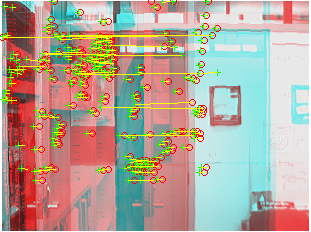
\includegraphics[width=0.8\linewidth]{Images/01_our_match.png}
	\caption{Interesting points and matches using our implementation on Image 1.}
	\label{fig:jp-ofc-ours-match}
\end{figure}

\begin{figure}[H]\centering
	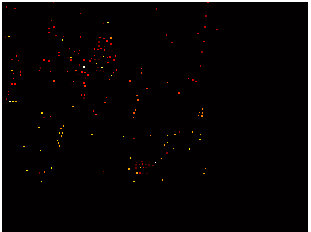
\includegraphics[width=0.8\linewidth]{Images/01_our_depth.png}
	\caption{Depth map using the interesting points and matches using our implementation on Image 1.}
	\label{fig:jp-ofc-ours-depth}
\end{figure}

% Image 2
\begin{figure}[H]\centering
	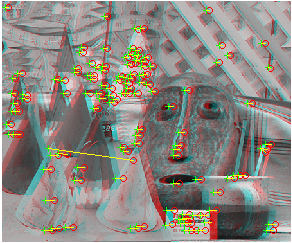
\includegraphics[width=0.8\linewidth]{Images/02_matlab_match.png}
	\caption{Interesting points and matches found using MATLAB's implementation on Image 2.}
	\label{fig:grid-example}
\end{figure}

\begin{figure}[H]\centering
	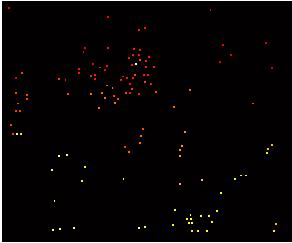
\includegraphics[width=0.8\linewidth]{Images/02_matlab_depth.png}
	\caption{Depth map using the interesting points and matches using MATLAB's implementation on Image 2.}
	\label{fig:grid-example}
\end{figure}

\begin{figure}[H]\centering
	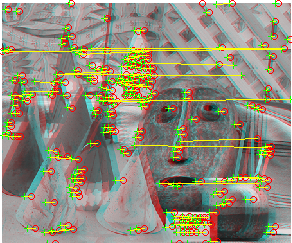
\includegraphics[width=0.8\linewidth]{Images/02_our_match.png}
	\caption{Interesting points and matches using our implementation on Image 2.}
	\label{fig:grid-example}
\end{figure}

\begin{figure}[H]\centering
	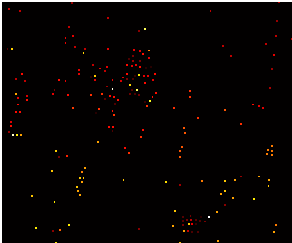
\includegraphics[width=0.8\linewidth]{Images/02_our_depth.png}
	\caption{Depth map using the interesting points and matches using our implementation on Image 2.}
	\label{fig:grid-example}
\end{figure}

% Image 3
\begin{figure}[H]\centering
	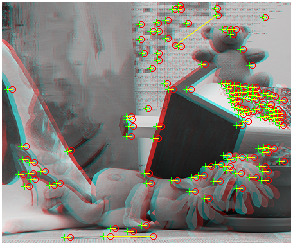
\includegraphics[width=0.8\linewidth]{Images/03_matlab_match.png}
	\caption{Interesting points and matches found using MATLAB's implementation on Image 3.}
	\label{fig:grid-example}
\end{figure}

\begin{figure}[H]\centering
	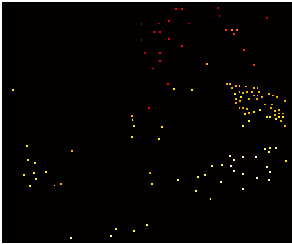
\includegraphics[width=0.8\linewidth]{Images/03_matlab_depth.png}
	\caption{Depth map using the interesting points and matches using MATLAB's implementation on Image 3.}
	\label{fig:grid-example}
\end{figure}

\begin{figure}[H]\centering
	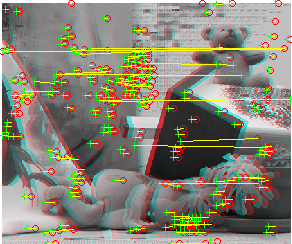
\includegraphics[width=0.8\linewidth]{Images/03_our_match.png}
	\caption{Interesting points and matches using our implementation on Image 3.}
	\label{fig:grid-example}
\end{figure}

\begin{figure}[H]\centering
	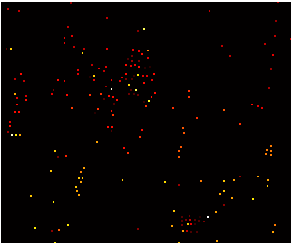
\includegraphics[width=0.8\linewidth]{Images/03_our_depth.png}
	\caption{Depth map using the interesting points and matches using our implementation on Image 3.}
	\label{fig:grid-example}
\end{figure}

As we can see from the result images, our implementation is reasonably close to the MATLAB point matching algorithm given the same corner data -- in the case of Figures \ref{fig:jp-ofc-matlab-match}-\ref{fig:jp-ofc-ours-depth}, our algorithm bested MATLAB's algorithm, finding significantly more matches. MATLAB's approach to matching features is similar to ours, matching using a 11x11 window (as per MATLAB's documentation). 

Our algorithm had the tendency to make matches that went across the image. In an attempt to stop these bogus matches, we weighted the match scores inversely proportional to the distance away from the point we were trying to find a match for. However, even with this weighting, it simply turned out that these matches were the best that the algorithm could find -- likely a result of being a greedy algorithm and just matching whatever points were left over. 